\subsection{2012 ANES}
% Here, we will look at political sophistication and competence

\begin{frame}\centering\vfill
    \begin{center}
        \begin{tikzpicture}
            \node[anchor=south west,inner sep=0] (image) at (0,0) {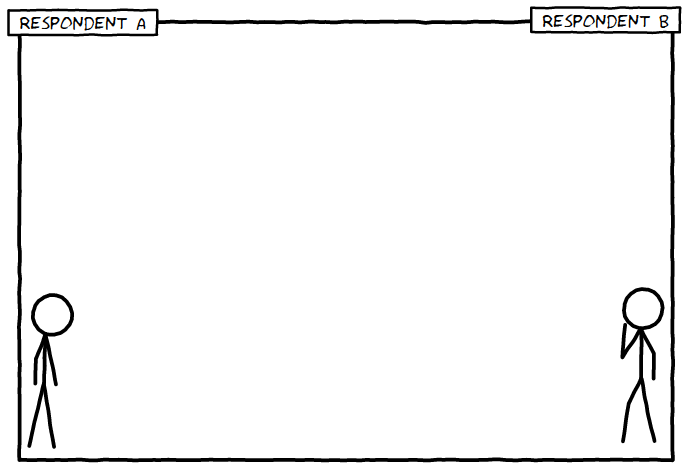
\includegraphics[width=\textwidth]{fig/Respondents_empty.png}};
            \node<2->[anchor=south west,inner sep=0] (vote) at (1.5,5) {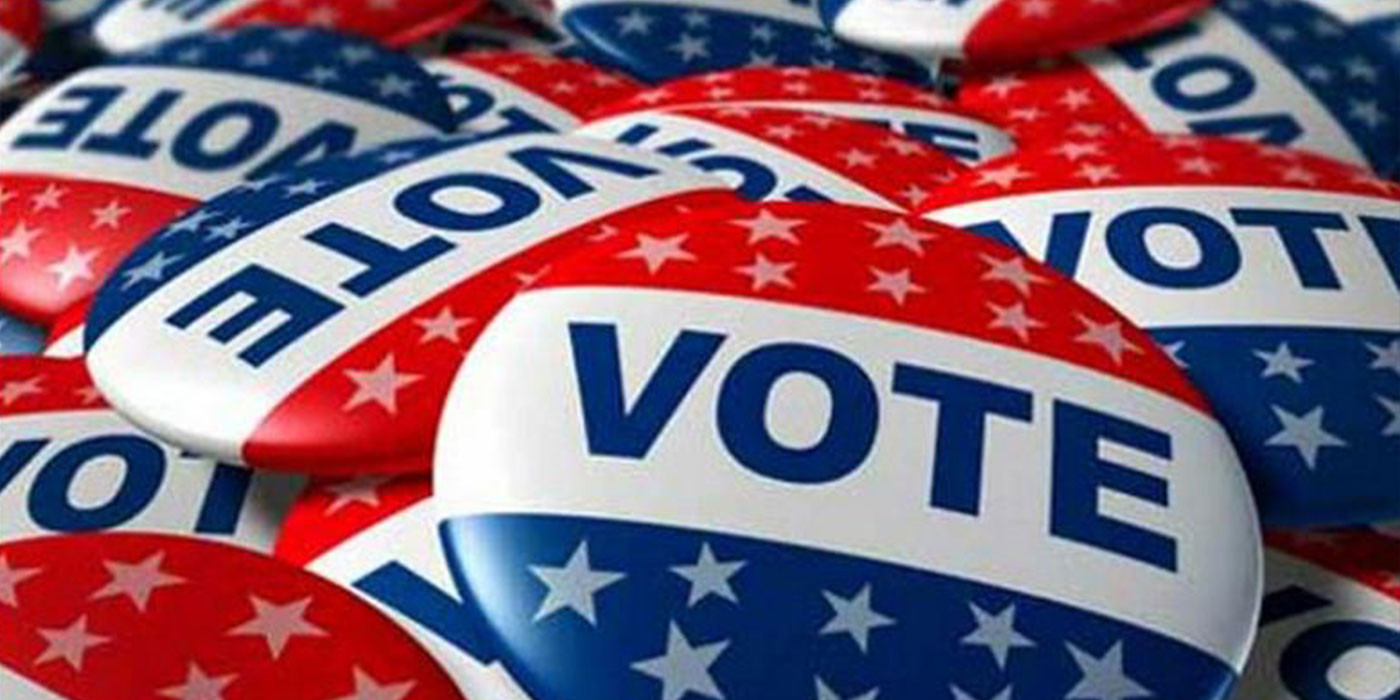
\includegraphics[width=.4\textwidth]{fig/Voting.jpg}};
            \node<3->[anchor=south west,inner sep=0] (protest) at (4.6,1.5) {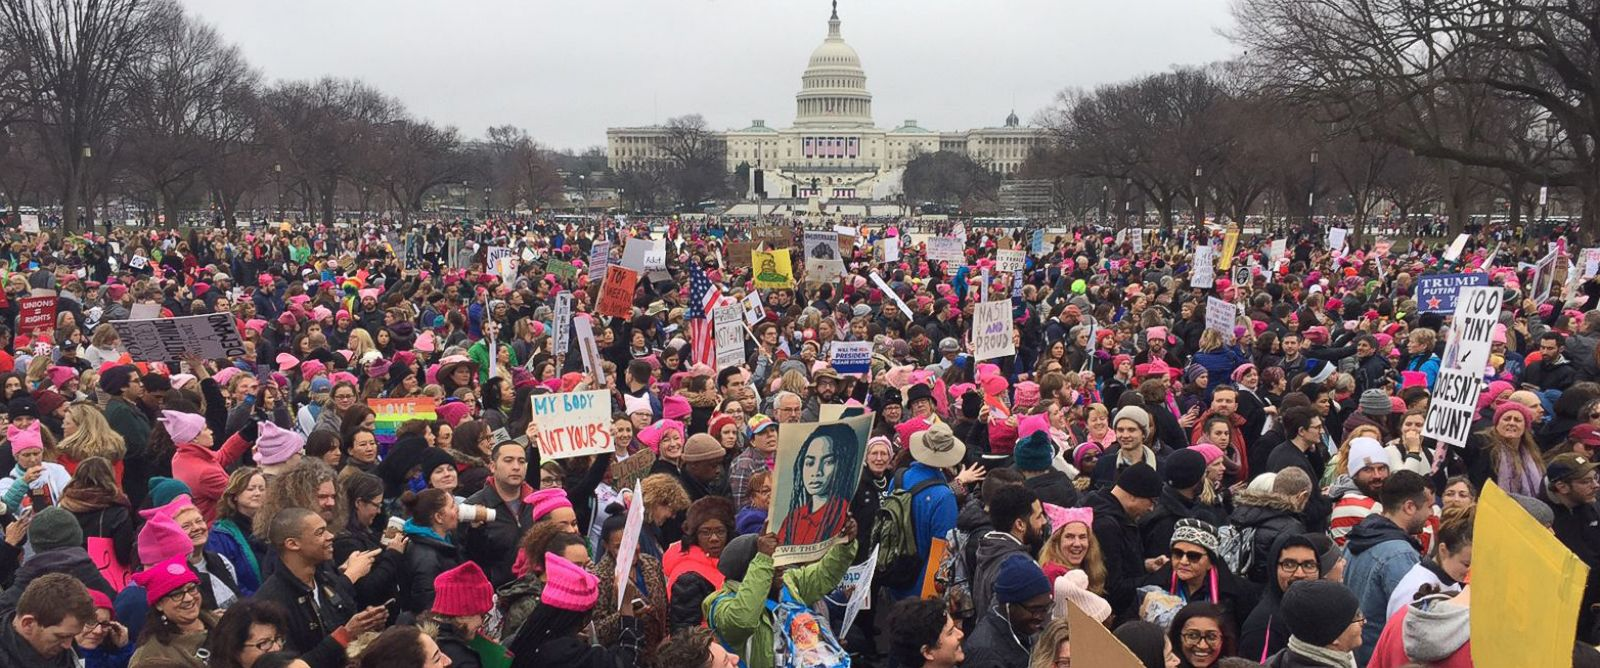
\includegraphics[width=.5\textwidth]{fig/GTY-womens-march.jpg}};
            \node<4->[anchor=south west,inner sep=0] (thinking) at (1.5,1.5) {
\includegraphics[width=.25\textwidth]{fig/gear-head-blue.png}};
            \node<5->[anchor=south west,inner sep=0] (influence) at (6.5,4.5) {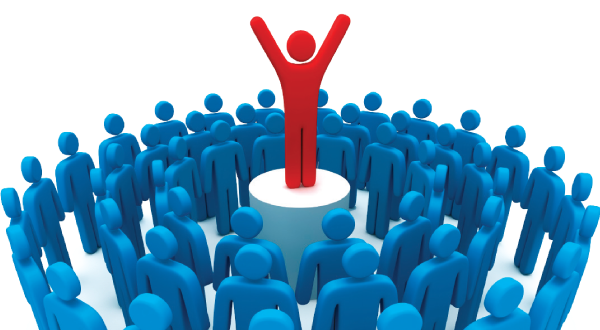
\includegraphics[width=.3\textwidth]{fig/Influence.png}};
            \node<6->[align=center,draw opacity=0,fill opacity=0.8,text opacity=1, white, fill=beamer@sbred] at (image.center) {\large Validation 1\\\Large 2012 American National Election Study\\\vspace{1em}\\N = 5914 (2054 f2f + 3860 online)};
        \end{tikzpicture}
    \end{center}
\end{frame}
%\item Non-response: 417, Spanish: 228

\begin{frame}{\hyperlink{engagement_joint}{Engagement and Participation}}\label{engagement}
  \begin{figure}
  \only<1>{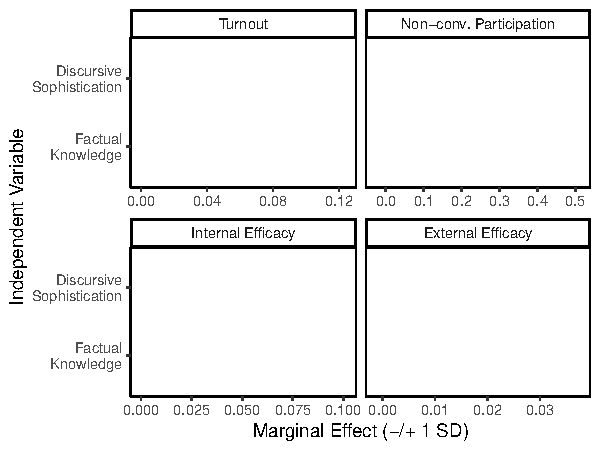
\includegraphics{../fig/knoweff_pres0.pdf}}
  \only<2>{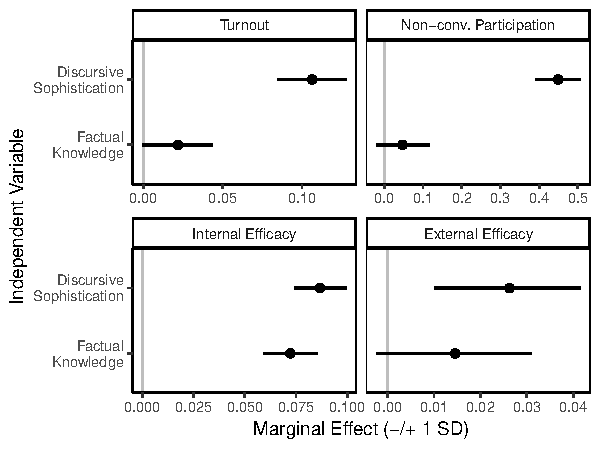
\includegraphics{../fig/knoweff_pres1.pdf}}
  \end{figure}
\end{frame}
% DISCUSS:
% Discursive sophistication is associated with:
% - \hyperlink{hetreg}{more precise candidate and party \emph{placements} on multiple \emph{policy} issues.
% -\hyperlink{prepost}{higher likelihood that citizens \emph{voted} according to their \emph{initial intention} at the time of the \emph{pre-election} interview.



\subsection{2015 YouGov Study}
% Here, we will look at political sophistication and competence
% Introduce the main point here!!


\begin{frame}\centering\vfill
\begin{center}
	\begin{tikzpicture}
	\node[anchor=south west,inner sep=0] (image) at (0,0) {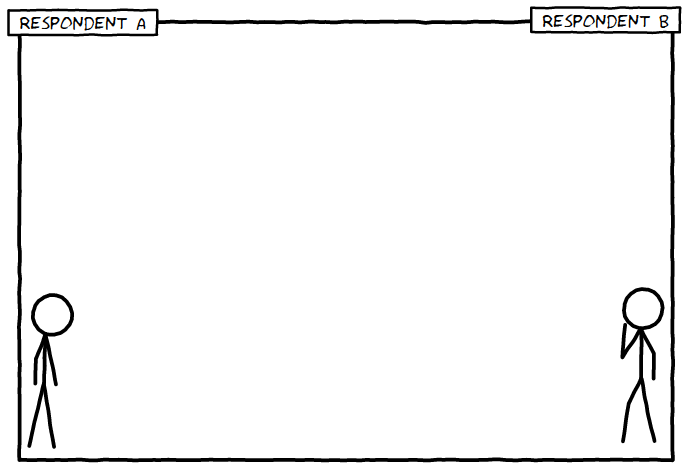
\includegraphics[width=\textwidth]{fig/Respondents_empty.png}};
	\node<2->[anchor=south west,inner sep=0] (information) at (3.6,1.2) {
\includegraphics[width=.4\textwidth]{fig/Information-mag-glass-1024x1024.jpg}};
	\node<3->[align=center,draw opacity=0,fill opacity=0.8,text opacity=1, white, fill=beamer@sbred] at (image.center) {\large Validation 2
		\\\Large 2015 YouGov Study
		\\\vspace{1em}\\ N = 1000 (online)};
	\end{tikzpicture}
\end{center}
\end{frame}
%Non-response: 48

\begin{frame} %[allowframebreaks]
\frametitle{\hyperlink{retrieval_joint}{Accurate Information Retrieval}}\label{retrieval}
\begin{figure}
\only<1>{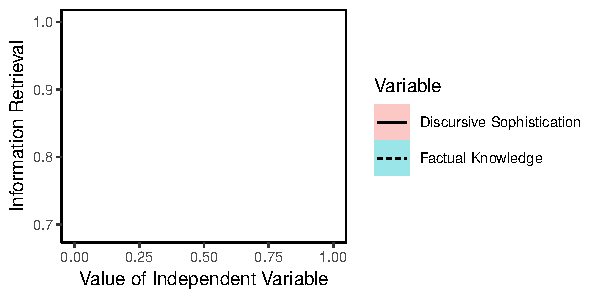
\includegraphics{../fig/yg_disease0.pdf}}
\only<2>{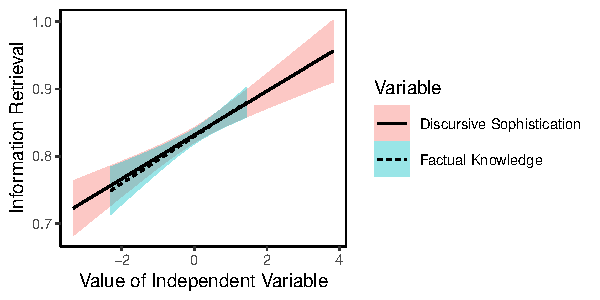
\includegraphics{../fig/yg_disease.pdf}}
\end{figure}
\end{frame}


\subsection{2008--2012 Swiss Referendum Survey}
% Here, we will look at political sophistication and competence
% Manual coding would be the ideal, Colombo as the gold standard

\begin{frame}\centering\vfill
\begin{center}
	\begin{tikzpicture}
	\node[anchor=south west,inner sep=0] (image) at (0,0) {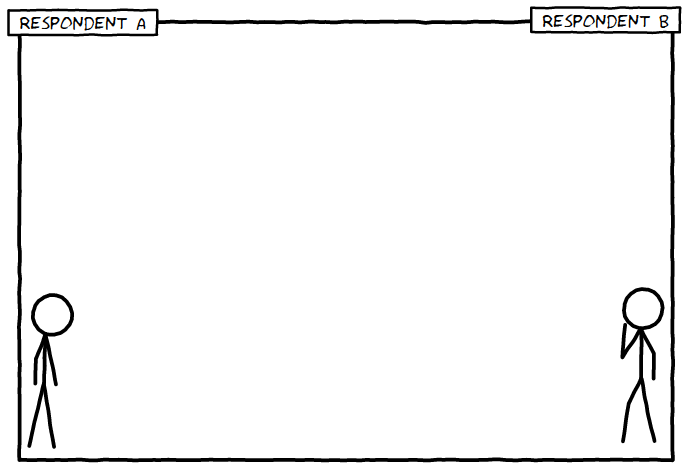
\includegraphics[width=\textwidth]{fig/Respondents_empty.png}};
	\node<2->[anchor=south west,inner sep=0] (circle) at (2.5,1) {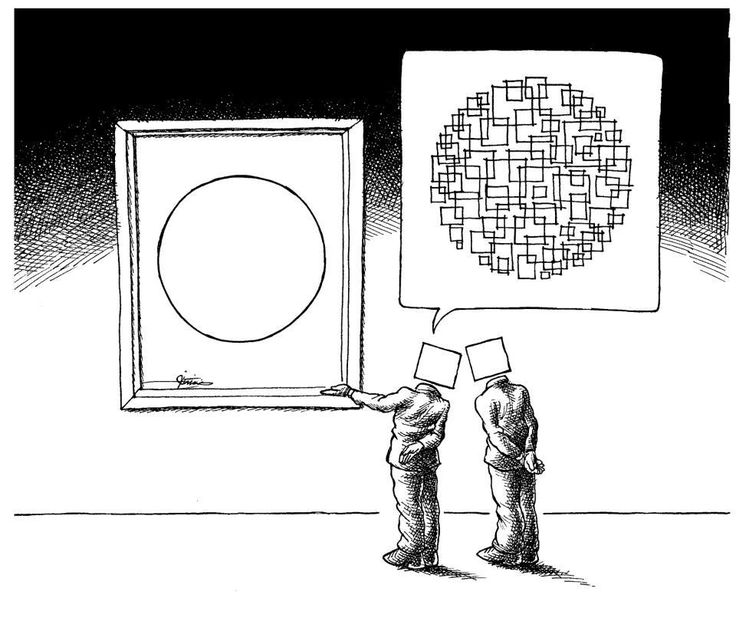
\includegraphics[width=.6\textwidth]{fig/circle.jpg}};
	\node<3->[align=center,draw opacity=0,fill opacity=0.8,text opacity=1, white, fill=beamer@sbred] at (image.center) {\large Validation 3
		\\\Large 2008--2012 Swiss Referendum Survey
		\\\large \citep{colombo2016justifications}
		\\\vspace{1em}\\N = 26,621 (phone)};
	\end{tikzpicture}
\end{center}
\end{frame}
%Non-response: 4,917

% Manually coding would be the gold standard... How would it compare across 3 different languages -> very hard test!!!

\begin{frame} %[allowframebreaks]
\frametitle{Comparison with Manually Coded Levels of Justification}
\begin{figure}
\only<1>{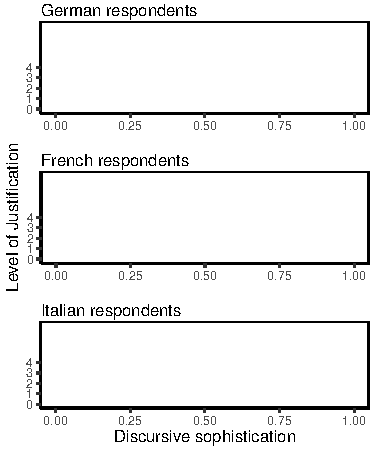
\includegraphics{../fig/swiss_ggridges_0.pdf}}\only<2>{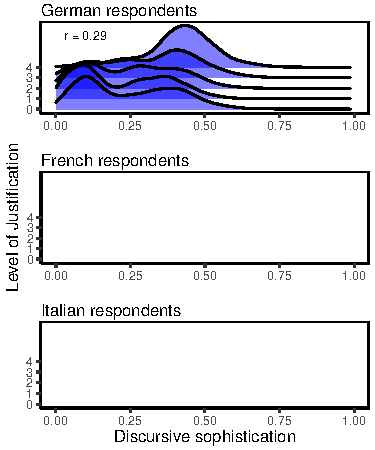
\includegraphics{../fig/swiss_ggridges_1.pdf}}\only<3>{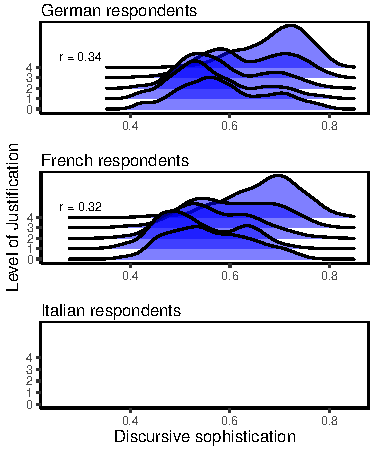
\includegraphics{../fig/swiss_ggridges_2.pdf}}\only<4>{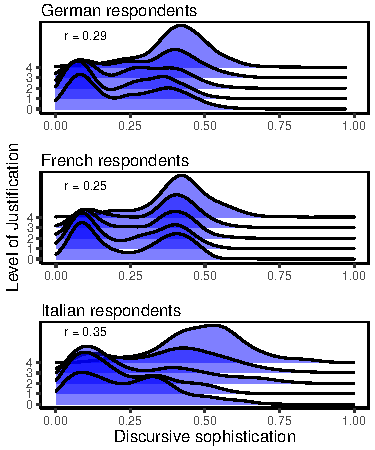
\includegraphics{../fig/swiss_ggridges_3.pdf}}
\end{figure}
\end{frame}




